%variant 62: 1976, 2


\begin{document}

\newpage

\renewcommand{\headrulewidth}{0.6pt}
\setcounter{page}{51}
\fancyhf{}
\fancyfoot[R]{\bfseries\thepage}
\rhead{kvant.mccme.ru}

\begin{multicols}{2}
\begin{flushleft}
    \textit{Г. Мякишев}
\end{flushleft}

\begin{flushleft}
    \Large \textbf{Расчет цепей \\ переменного тока \\ с помощью \\ векторных диаграмм}
\end{flushleft}

\begin{flushleft}
    Расчет цепей переменного тока значительно сложнее, чем цепей постоянного тока. Однако в случае, если напряжение и сила тока изменяются по гармоническому закону, существует довольно простой и наглядный метод расчета цепей - метод векторных диаграмм. С ним мы и хотим познакомить читателей в этой статье.
\end{flushleft}

\begin{flushleft}
    \textbf{Уравнение, \\ описывающее вынужденные колебания в колебательном контуре}
\end{flushleft}
Промышленный переменный ток - это вынужденные электромагнитные колебания. Если напряжение $u = u(t)$ на концах цепи меняется по гармоническому закону
\begin{center} $u = U_0cos\omega t$, (1) \end{center}

\noindent то сила тока $i$ также меняется гармонически с той же частотой $\omega$, но в общем случае ток сдвинут по фазе относительно напряжения на постоянную величину $\phi$:
\begin{center}
    $i=I_0cos(\omega t + \phi)$. (2)
\end{center}

\indent Впрочем, в первый момент после замыкания цепи колебания тока имеют гораздо более сложную форму. При замыкании электрическая цепь как бы получает «толчок», и если она обладает собственной частотой колебаний $\omega_0$, то в ней возникают свободные электромагнитные колебания. Эти колебания накладываются на выну-

\columnbreak

\noindent
 жденные колебания частоты $\omega$, но постепенно затухают из-за наличия в цепи активного сопротивления $R$ (на котором происходит выделение энергии в виде тепла). Лишь после того как свободные колебания затухнут, вынужденные колебания можно считать установившимися. Амплитуда силы тока $I_0$ в формуле (2) - это амплитуда установившихся колебаний. Все происходит точно так же, как и в случае вынужденных механических колебаний (более подробно об этом см., например в статье \texttt{Г. Я. Мякишева} «Вынужденные механические колебания», «Квант», 1974, № 11).

\indent Довольно простой, но очень важный частный случай представляют собой вынужденные колебания в цепи, состоящей из последовательно соединенных проводника с активным сопротивлением $R$, катушки индуктивности $L$ и конденсатора емкости $C$ (рис. 1). Такую цепь называют по- следовательным колебательным контуром. Пусть напряжение $u$ на концах цепи меняется по закону, описываемому уравнением (1); тогда сила тока $i$ в цепи меняется в соответствии с выражением (2). Чему равна амплитуда тока $I_0$, и сдвиг фаз $\phi$?
Как известно, уравнение, описывающее вынужденные колебания тока в этом контуре, имеет следующий вид:
\begin{center}
    $L\frac{\Delta i}{\Delta t} + Ri + \frac{q}{C} = U_0cos\omega t$. (3)
\end{center}
Здесь $q$ - заряд конденсатора. (Это

\begin{flushleft}
    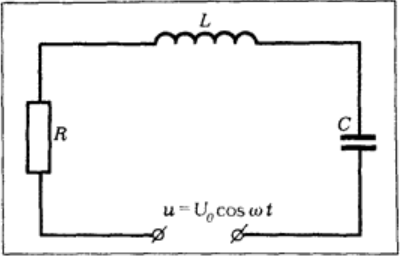
\includegraphics[width=\linewidth]{img.png}
    \small \bfseries Рис. 1.
\end{flushleft}

\end{multicols}

\end{document}